% !TEX program = pdflatex
\documentclass[10pt,conference,letterpaper]{IEEEtran}

\usepackage[utf8]{inputenc}
\usepackage[T1]{fontenc}
\usepackage{booktabs}
\usepackage{graphicx}
\usepackage{hyperref}
\usepackage{listings}
\usepackage{xcolor}
\usepackage{amsmath,amssymb}
\usepackage{enumitem}
\usepackage{caption}
\usepackage{multirow}
\usepackage{array}
\usepackage{url}
\usepackage{tikz}
\usetikzlibrary{shapes.geometric, arrows.meta, positioning, calc, fit}

% Hyperref setup
\hypersetup{
    colorlinks=true,
    linkcolor=blue!60!black,
    citecolor=blue!60!black,
    urlcolor=blue!60!black,
    bookmarks=true,
    pdftitle={Budgeted End-to-End LLM4HLS Agent},
    pdfauthor={Anonymous},
    pdfsubject={LLM4HLS Agent for Vitis HLS},
    pdfkeywords={HLS, LLM, FPGA, Vitis, Agent}
}

% Listings setup for C++ code
\definecolor{codebg}{RGB}{248,248,248}
\definecolor{codekw}{RGB}{0,0,180}
\definecolor{codecm}{RGB}{0,128,0}
\definecolor{codestr}{RGB}{163,21,21}
\lstset{
    language=C++,
    basicstyle=\ttfamily\footnotesize,
    keywordstyle=\color{codekw}\bfseries,
    commentstyle=\color{codecm}\itshape,
    stringstyle=\color{codestr},
    backgroundcolor=\color{codebg},
    frame=single,
    framerule=0.4pt,
    rulecolor=\color{gray!50},
    numbers=left,
    numberstyle=\tiny\color{gray},
    numbersep=6pt,
    breaklines=true,
    showstringspaces=false,
    captionpos=b,
    tabsize=2,
    columns=fullflexible,
    keepspaces=true,
    morekeywords={pragma, HLS, PIPELINE, UNROLL, ARRAY_PARTITION, DATAFLOW,
                   hls, stream, ap_int, ap_uint}
}

% Compact lists
\setlist{nosep, leftmargin=1.2em}

\begin{document}

\title{Budgeted End-to-End LLM4HLS Agent: \\
Automated Repair and Optimization of Vitis HLS Code \\
within Constrained Tool-Call Budgets}

\author{
\IEEEauthorblockN{Anonymous}
\IEEEauthorblockA{Submitted to FPT'26 Design Competition -- Track A: LLM4HLS Agent}
}

\maketitle

\begin{abstract}
We present an autonomous AI agent that repairs and optimizes AMD Vitis HLS C/C++ kernels under a constrained tool-invocation budget. The agent receives an HLS task---possibly containing a functional bug, a synthesis failure, a co-simulation deadlock, or merely an unoptimized baseline---and iteratively drives it to functional correctness before optimizing its PPA (Performance--Power--Area). The architecture follows a linear-with-backtracking three-stage flow: \emph{correctness repair} $\rightarrow$ \emph{synthesis verification} $\rightarrow$ \emph{PPA optimization}, where every code edit re-verifies already-passed stages and a monotone checkpoint archive provides rollback for free. The optimization stage implements the AMD LLM4HLS four-phase workflow: design-brief extraction, strategy proposal with compatibility annotations, a reviewer-AI dual-confirmation gate, and combined code generation. A deterministic mechanical-check gate complements LLM self-review to catch signature changes that the LLM misses. We evaluate on six tasks spanning three task types (repair, structural, optimize) on Vitis 2025.2 targeting Alveo U55C at 200\,MHz with all three competition-recommended open-weight models (DeepSeek V4 Pro, Qwen3.5 122B, Qwen3.6 27B): every model clears the csim correctness gate on all six tasks (18/18), demonstrating that the architecture transfers across models without modification. With DeepSeek V4 Pro the agent achieves two perfect scores and up to 205$\times$ latency reduction; all candidates close timing with conservative Fmax of 200--353\,MHz at a maximum resource utilization of 3.5\%. A graded token-mode A/B study shows 8--31\% token savings without score degradation. All artifacts are packaged as a reproducible Docker image, and all experiment data are archived for auditability.
\end{abstract}

\begin{IEEEkeywords}
High-Level Synthesis, LLM agents, Vitis HLS, FPGA, correctness-first optimization, budgeted tool use
\end{IEEEkeywords}

% ============================================================
\section{Introduction}
% ============================================================

Writing correct HLS code requires simultaneously managing algorithm correctness and hardware constraints; a misplaced \texttt{\#pragma} can cause synthesis failure or co-simulation deadlock. Directly prompting an LLM to ``write correct HLS'' in one shot rarely succeeds; an iterative loop with tool feedback is necessary~\cite{react,autochip,hlsrepair}. FPT'26 Track A formalizes this: build an autonomous agent that, under a bounded tool-call budget, repairs and optimizes HLS tasks~\cite{fpt26rules}. Scoring uses a hidden testbench with a correctness gate (Eq.~\ref{eq:score}): correctness carries 0.5 weight (hard gate), synthesis 0.2, and PPA acceleration (capped at 8$\times$, latency-only) 0.3. Token consumption is an explicit evaluation factor.

Our contributions: (1) a \textbf{three-stage architecture} (correctness $\rightarrow$ synth $\rightarrow$ optimize) with backtracking re-verification and a monotone checkpoint archive (\S\ref{sec:arch}); (2) an \textbf{AMD four-phase optimization workflow}---design-brief extraction, strategy proposal, reviewer-AI dual-confirmation, combined application~\cite{amdllm4hls} (\S\ref{sec:optimize}); (3) a \textbf{dual-gate review} where deterministic mechanical checks catch signature changes that LLM self-review misses; (4) a \textbf{graded token-saving switch} saving 8--31\% tokens without score loss; (5) \textbf{multi-model validation} on six tasks with three competition-recommended open-weight models.

% ============================================================
\section{System Architecture}
\label{sec:arch}
% ============================================================

The agent follows a \emph{linear flow with backtracking re-verification and checkpoint arbitration} (Fig.~\ref{fig:overview}). A router reads \texttt{task.toml} at zero credit cost and selects the stage path. The checkpoint maps stage completion to a monotone level (Lv0: nothing $\to$ Lv1: csim+pass $\to$ Lv2: +synth pass), with three archive rules: level-up $\to$ accept; same-level $\to$ lower latency wins; level-down $\to$ reject (auto-rollback). Every code edit passes a dual gate: deterministic mechanical checks (signature/include) followed by LLM self-review. Stage 1 runs a repair loop (csim fail $\to$ feedback $\to$ KB retrieval $\to$ LLM repair $\to$ dual-gate $\to$ retry). Stage 2 re-verifies csim before each synth (1 credit $<$ 4 credits). Stage 3 implements the AMD four-phase workflow: extract design brief $\to$ propose strategies with compatibility annotations $\to$ reviewer-AI dual-confirmation $\to$ combined application, with credit-driven stopping. A post-optimization cosim re-check with repair-then-rollback guards against shipping deadlocks. Detailed algorithms, stopping policies, and the knowledge base (22 bug$\to$fix entries) are in Appendix~\ref{app:algorithms}--\ref{app:kb}.

\begin{figure}[t]
\centering
\resizebox{\linewidth}{!}{%
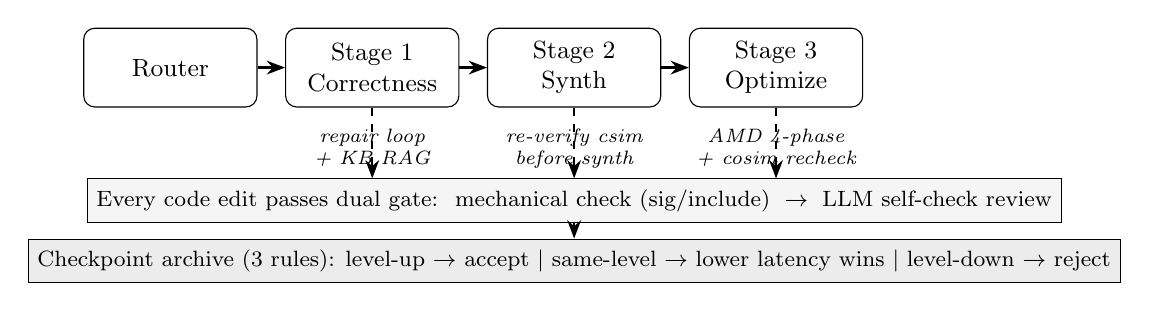
\begin{tikzpicture}[
  node distance=0.3cm and 0.35cm,
  stage/.style={draw, rounded corners, minimum height=1.0cm, minimum width=2.2cm, align=center, font=\small},
  sub/.style={font=\scriptsize\itshape, align=center, text width=2.2cm},
  bar/.style={draw, minimum height=0.55cm, align=center, font=\footnotesize, fill=gray!8},
  arrow/.style={-Stealth, thick},
  every node/.style={font=\small}
]
\node[stage] (router) {Router};
\node[stage, right=of router] (s1) {Stage 1\\Correctness};
\node[stage, right=of s1] (s2) {Stage 2\\Synth};
\node[stage, right=of s2] (s3) {Stage 3\\Optimize};

\draw[arrow] (router) -- (s1);
\draw[arrow] (s1) -- (s2);
\draw[arrow] (s2) -- (s3);

\node[sub, below=0.15cm of s1] {repair loop\\+ KB RAG};
\node[sub, below=0.15cm of s2] {re-verify csim\\before synth};
\node[sub, below=0.15cm of s3] {AMD 4-phase\\+ cosim recheck};

\node[bar, below=0.9cm of s2, minimum width=9.5cm] (gate)
  {Every code edit passes dual gate: \;mechanical check (sig/include) \;$\to$\; LLM self-check review};

\node[bar, below=0.2cm of gate, minimum width=9.5cm, fill=gray!15] (ckpt)
  {Checkpoint archive (3 rules): level-up $\to$ accept $|$ same-level $\to$ lower latency wins $|$ level-down $\to$ reject};

\draw[arrow, dashed] (s1.south) -- ++(0,-0.25) -| (gate.north -| s1.south);
\draw[arrow, dashed] (s2.south) -- (gate.north -| s2.south);
\draw[arrow, dashed] (s3.south) -- ++(0,-0.25) -| (gate.north -| s3.south);
\draw[arrow] (gate) -- (ckpt);
\end{tikzpicture}%
}
\caption{Agent architecture. Three stages run sequentially; every code edit passes a dual review gate before the checkpoint arbitrates. The monotone-level rule gives automatic rollback.}
\label{fig:overview}
\end{figure}

% ============================================================
\section{Experiments}
\label{sec:results}
% ============================================================

All runs use Vitis 2025.2~\cite{ug1399} targeting Alveo U55C \texttt{xcu55c-fsvh2892-2L-e} @ 200\,MHz (5\,ns). Scoring uses the official \texttt{grade()} on hidden testbenches. We evaluate three competition-recommended models~\cite{fpt26rules,deepseek,qwen}: DeepSeek V4 Pro (1.6T MoE), Qwen3.5 122B A10B, and Qwen3.6 27B, on six tasks (three official + three self-built). Setup details and the task suite are in Appendix~\ref{app:setup}.

\subsection{Main Results (DeepSeek V4 Pro)}

\begin{table}[h]
\centering
\caption{End-to-end results (DeepSeek V4 Pro, best archived run). Correctness 6/6 = 100\%.}
\label{tab:results}
\footnotesize
\begin{tabular}{lclrrrr}
\toprule
\textbf{Task} & \textbf{Diff.} & \textbf{SCORE} & \textbf{Cand lat.} & \textbf{Accel.} & \textbf{Cr.} & \textbf{Tokens} \\
\midrule
projection & 2 & \textbf{1.400} & 0$^\dagger$ & --- & 5 & 3,629 \\
residual & 4 & \textbf{4.000} & 10 & 13.5$\times$ & 65 & 77,754 \\
dotProduct & 3 & \textbf{3.000} & 20 & 51.35$\times$ & 40 & 67,253 \\
matmul & 3 & \textbf{2.691} & 3,126 & 5.25$\times$ & 35 & 50,729 \\
fir & 2 & \textbf{2.000} & 542 & 30.5$\times$ & 40 & 127,162 \\
vecadd & 1 & \textbf{1.000} & 20 & 205$\times$ & 20 & 46,924 \\
\bottomrule
\end{tabular}
\\[2pt]
\scriptsize $^\dagger$Combinational logic (latency=0); PPA slice unreachable (\S\ref{app:harness-quirk}).
\end{table}

Two tasks achieve perfect scores (residual 4.000, dotProduct 3.000). All candidates close timing (Fmax 200--353\,MHz, well above the 100\,MHz rule) at $\leq$3.5\% resource utilization. Full PPA data is in Appendix~\ref{app:ppa}.

\subsection{Multi-Model Comparison (Contest Rule 6)}
\label{sec:multimodel}

\begin{table}[h]
\centering
\caption{Multi-model comparison (one run per model/task, token-mode \texttt{full}).}
\label{tab:multimodel}
\scriptsize
\begin{tabular}{l rrr rrr rrr}
\toprule
& \multicolumn{3}{c}{\textbf{DeepSeek V4 Pro}} & \multicolumn{3}{c}{\textbf{Qwen3.5 122B}} & \multicolumn{3}{c}{\textbf{Qwen3.6 27B}} \\
\cmidrule(lr){2-4} \cmidrule(lr){5-7} \cmidrule(lr){8-10}
\textbf{Task} & \textbf{Scr} & \textbf{Cr} & \textbf{Tok} & \textbf{Scr} & \textbf{Cr} & \textbf{Tok} & \textbf{Scr} & \textbf{Cr} & \textbf{Tok} \\
\midrule
projection & 1.4 & 5 & 3.6k & 1.4 & 5 & 15.1k & 1.4 & 5 & 13.9k \\
residual & \textbf{4.0} & 65 & 77.8k & 3.1 & 30 & 42.0k & 3.4 & 60 & 68.4k \\
dotProduct & \textbf{3.0} & 40 & 67.3k & \textbf{3.0} & 15 & 72.8k & 2.3 & 10 & 38.5k \\
matmul & 2.7 & 35 & 50.7k & 2.2 & 10 & 67.5k & \textbf{3.0} & 30 & 54.5k \\
fir & \textbf{2.0} & 40 & 127.2k & \textbf{2.0} & 30 & 152.2k & 1.5 & 25 & 64.3k \\
vecadd & \textbf{1.0} & 20 & 46.9k & 0.5 & 20 & 59.7k & 0.7 & 20 & 37.7k \\
\midrule
\textbf{Total} & \multicolumn{3}{r}{14.1 / 373k} & \multicolumn{3}{r}{12.2 / 409k} & \multicolumn{3}{r}{12.3 / 277k} \\
\bottomrule
\end{tabular}
\end{table}

All three models clear the csim correctness gate on all six tasks (18/18)---the correctness-first architecture is model-agnostic. Optimization quality varies: Qwen3.6 27B produced the only perfect matmul (210$\times$) while stalling on vecadd; DeepSeek achieves the best score/token trade-off. A graded token-mode switch (\texttt{balanced}) saves 8--31\% tokens without score loss (Appendix~\ref{app:tokens}). Variance and failure-mode analysis is in Appendix~\ref{app:variance}.

% ============================================================
\section{Discussion}
% ============================================================

The scored PPA term is $p=\min(\text{Accel},8)/8$---latency-only. Under this metric, latency-first optimization is score-optimal; area/power reduction has zero marginal value. We guard against the two failure modes: area explosion is caught by the reviewer-AI feasibility gate, and timing failure is prevented by the 5\,ns synthesis target. Detailed design rationale, a harness edge case (zero-latency scoring), limitations, and future work are in Appendix~\ref{app:discussion}.

% ============================================================
\section{Related Work}
% ============================================================

ReAct~\cite{react} interleaves reasoning with tool actions; our agent instantiates this loop in the HLS domain. HLS-Repair~\cite{hlsrepair} and HLSPilot~\cite{hlspilot} repair/automate HLS with LLMs but stop at correctness; we couple repair with PPA optimization under a hard budget. AMD's case study~\cite{amdllm4hls} proposes a human-in-the-loop four-phase workflow; we engineer it into a fully autonomous loop. Extended related work is in Appendix~\ref{app:related}.

% ============================================================
\section{Conclusion}
% ============================================================

We built a budgeted end-to-end LLM4HLS agent achieving 100\% correctness (18/18 across three models), two perfect scores, and up to 205$\times$ latency reduction on six tasks with Vitis 2025.2 + Alveo U55C. The core design---three-stage architecture, AMD four-phase optimization, dual-gate review, and graded token saving---transfers across models without modification and is packaged as a reproducible Docker submission.

% ============================================================
\bibliographystyle{IEEEtran}
\bibliography{report}

\appendix

% ============================================================
\section{Detailed Algorithms}
\label{app:algorithms}
% ============================================================

\subsection{Stage 1: Correctness Repair Loop}
\label{sec:correctness}

Goal: pass all correctness-gate stages. Each iteration:
\begin{enumerate}
    \item \textbf{Pre-csim LLM review} (first attempt only): before spending a credit on csim, let the LLM inspect the code and fix obvious bugs. On the \texttt{residual\_stream\_deadlock} task, this step identified and fixed the DATAFLOW deadlock pattern \emph{before} any tool call---saving a 20-credit failed cosim and a 15-minute timeout.
    \item Run csim (+ cosim if structural).
    \item Pass $\to$ archive to Lv1, proceed to Stage 2.
    \item Fail $\to$ distill feedback $\to$ KB retrieval $\to$ repair $\to$ dual-gate review $\to$ retry.
\end{enumerate}

\textbf{Dual-gate review} (applied at every code edit):
\begin{itemize}
    \item \emph{Gate 1 -- Mechanical checks} (deterministic, non-LLM): verify the top-level function signature is unchanged and the header \texttt{\#include} is still present. In one observed instance, the LLM self-check approved a candidate whose top-level signature had changed (which would fail hidden-testbench linking); the mechanical gate caught it.
    \item \emph{Gate 2 -- LLM self-check review}: same model, reviewer prompt, checking interface/new bugs/pragma hazards. A rejection triggers re-generation.
\end{itemize}

\subsection{Stage 2: Synthesis Verification}

Goal: verify synthesizability and obtain baseline latency. On synth failure, a repair loop runs, but each edit re-verifies csim (1 credit) before spending another synth (4 credits). The loop runs up to \texttt{max\_synth\_rounds}=3. A latency validity defense treats $\leq 0$ as missing data, preventing a ``0-cycle'' design from corrupting the archive.

\subsection{Stage 3: PPA Optimization --- AMD Four-Phase Workflow}
\label{sec:optimize}

\paragraph{Phase 1 -- Context Loading.} Official design document + design brief extraction (LLM\#3, cached) + synthesis report + device constraints + checkpoint snapshot.

\paragraph{Phase 2a -- Strategy Proposal (LLM\#4).} Proposes 2--4 strategies, each annotated with \texttt{combinable\_with}. Uses JSON structured output.

\paragraph{Phase 2b -- Reviewer AI (LLM\#5).} Two steps: (1) feasibility review per strategy (interface unchanged, functionality preserved, synthesizable, resources fit); (2) compatibility re-check. The \emph{proposer} and \emph{reviewer} must both agree before combination.

\paragraph{Phase 3 -- Combined Application (LLM\#6).} Selected subset applied as one candidate, passing dual-gate review, then re-verifying csim + synth.

\textbf{Stopping policy} (credit-driven): convergence (not strictly faster $\to$ stop); credit exhaustion; credit reservation for structural tasks (26 credits for final cosim re-check); safety round cap (20).

\subsection{Post-Optimization Co-Simulation Re-check}
\label{sec:cosim-recheck}

After optimization, a final RTL sanity check runs for all task types. If best changed and cosim is affordable: pass $\to$ mark \texttt{cosim\_ok}; fail $\to$ repair-then-rollback (repair with cosim feedback, up to 3 retries, then rollback to pre-optimization snapshot).

% ============================================================
\section{Experiment Setup}
\label{app:setup}
% ============================================================

\paragraph{Hardware and software.} Ubuntu 22.04 server (8-core / 32\,GB), Vitis 2025.2, csim/synth/cosim via \texttt{vitis-run --mode hls}. Target: Alveo U55C \texttt{xcu55c-fsvh2892-2L-e}, 200\,MHz (5\,ns) clock. Scoring uses hidden testbenches outside the agent budget. All raw artifacts archived in \texttt{experiments/}.

\paragraph{Models.} DeepSeek V4 Pro (1.6T MoE, FP8; official API), Qwen3.5 122B A10B (AWQ-4bit), Qwen3.6 27B (FP8) (both via OpenAI-compatible MaaS). Temperature 0.2, token-mode \texttt{full} unless stated.

\paragraph{Protocol.} Each (model, task) pair run once; DeepSeek V4 Pro additionally has repeat runs for variance analysis. One exception: first Qwen3.5 matmul run died to LLM-API timeout and was re-run once with longer timeout.

\begin{table}[h]
\centering
\caption{Task suite. First three are official public tasks; last three are self-built.}
\label{tab:tasks}
\small
\begin{tabular}{>{\raggedright\arraybackslash}p{0.14\linewidth} l c c p{0.34\linewidth}}
\toprule
\textbf{Task} & \textbf{Type} & \textbf{Diff.} & \textbf{Bud.} & \textbf{Initial condition} \\
\midrule
projection & repair & 2 & 20 & csim fails: angle==0 branch drops vertex term \\
residual & struct. & 4 & 80 & csim ok, cosim deadlocks (FIFO burst) \\
dotProduct & optimize & 3 & 40 & correct, no pragmas \\
matmul & optimize & 3 & 60 & 32$\times$32 matmul, no pragmas \\
fir & optimize & 2 & 40 & 32-tap FIR, no pragmas \\
vecadd & optimize & 1 & 20 & vector add, no pragmas \\
\bottomrule
\end{tabular}
\end{table}

\subsection{Metered Tool Interface}

The harness provides \texttt{ToolServer} with three budget-charged calls: \texttt{csim}=1 credit, \texttt{synth}=4 credits, \texttt{cosim}=20 credits. Each task's budget is in \texttt{task.toml}. Credits do not accumulate across tasks.

\subsection{Scoring Formula}

\begin{equation}
\label{eq:score}
\text{score} = \begin{cases}
0 & \text{if not functional\_pass} \\
\text{diff} \times (0.5\,c + 0.2\,s + 0.3\,p) & \text{otherwise}
\end{cases}
\end{equation}
where $c=1$ if hidden csim (+cosim if required) passes, $s=1$ if synthesizable, $p = \min(\text{Accel}, 8)/8$.

\subsection{Task Types}

\begin{table}[h]
\centering
\caption{Task types and correctness gates.}
\label{tab:tasktypes}
\small
\begin{tabular}{lll}
\toprule
\textbf{task\_type} & \textbf{Typical initial state} & \textbf{Correctness gate} \\
\midrule
repair & csim fails (functional bug) & csim \\
optimize & csim passes, just slow & csim \\
structural & csim passes, cosim deadlocks & csim + cosim \\
generate & generate from scratch & csim (+cosim) \\
\bottomrule
\end{tabular}
\end{table}

% ============================================================
\section{Full PPA Report}
\label{app:ppa}
% ============================================================

\begin{table*}[t]
\centering
\caption{Full-PPA report of submitted candidates (DeepSeek V4 Pro), from Vitis csynth reports. Conservative Fmax $=1000/(\text{est}+\text{unc})$; all meet timing ($\geq$100\,MHz).}
\label{tab:ppa}
\footnotesize
\begin{tabular}{lrrc rrrr c}
\toprule
\textbf{Task} & \textbf{Lat.\ (cyc)} & \textbf{Est.\ clk (ns)} & \textbf{Fmax (MHz)} & \textbf{LUT} & \textbf{FF} & \textbf{BRAM-18K} & \textbf{DSP} & \textbf{Timing} \\
\midrule
projection & 0 & 2.54 & 257 & 692 / 1.30M (0.05\%) & 0 & 0 / 4032 & 0 / 9024 & \checkmark \\
residual & 10 & 1.48 & 353 & 366 (0.03\%) & 14 & 0 & 0 & \checkmark \\
dotProduct & 20$^\ddagger$ & 3.17 & 221 & 1,809 (0.14\%) & 1,135 & 0 & 64 (0.7\%) & \checkmark \\
matmul & 3,126 & 3.65 & 200 & 14,847 (1.1\%) & 18,018 & 10 (0.2\%) & 158 (1.8\%) & \checkmark \\
fir & 542 & 2.98 & 231 & 19,033 (1.5\%) & 27,041 & 0 & 316 (3.5\%) & \checkmark \\
vecadd & 262$^\S$ & 2.98 & 231 & 3,612 (0.3\%) & 3,377 & 0 & 32 (0.4\%) & \checkmark \\
\bottomrule
\end{tabular}
\\[3pt]
\footnotesize $^\ddagger$Latency 20 is best archived run; PPA row from latest run (identical structure). $^\S$vecadd from clean re-run.
\end{table*}

% ============================================================
\section{Token Efficiency}
\label{app:tokens}
% ============================================================

$\sim$89\% of completion tokens are reasoning tokens in reasoning models---the dominant cost. We implemented a graded \texttt{-{}-token-mode} switch:

\begin{table}[h]
\centering
\caption{Token-mode policy.}
\label{tab:tokenmode}
\small
\begin{tabular}{lp{0.6\linewidth}}
\toprule
\textbf{Mode} & \textbf{Settings} \\
\midrule
full (default) & No effort override \\
balanced & \texttt{review=off}, \texttt{select=off} \\
aggressive & Above + \texttt{brief=off}, \texttt{propose=off} \\
\bottomrule
\end{tabular}
\end{table}

\begin{table}[h]
\centering
\caption{Token-mode A/B study (full vs.\ balanced).}
\label{tab:ab}
\small
\begin{tabular}{lrrll}
\toprule
\textbf{Task} & \textbf{full tok.} & \textbf{bal.\ tok.} & \textbf{$\Delta$} & \textbf{SCORE (f$\to$b)} \\
\midrule
vecadd & 68,279 & 46,924 & $-$31.3\% & 1.000 $\to$ 1.000 \\
matmul & 55,357 & 50,729 & $-$8.4\% & 2.270 $\to$ 2.691 \\
dotProduct & 67,253 & 48,146 & $-$28.4\% & 3.000 $\to$ 3.000 \\
\bottomrule
\end{tabular}
\end{table}

Balanced mode saved 8--31\% tokens (mean 22.7\%) with no score degradation. The score--token frontier: vecadd \texttt{full} 68k $\to$ 1.000; \texttt{balanced} 47k $\to$ 1.000; \texttt{aggressive} 17k ($-$75\%) $\to$ 0.737. Strategy-proposal reasoning is where optimization quality comes from.

% ============================================================
\section{Run-to-Run Variance and Failure Modes}
\label{app:variance}
% ============================================================

\begin{table}[h]
\centering
\caption{Archived repeat runs (DeepSeek V4 Pro).}
\label{tab:variance}
\footnotesize
\begin{tabular}{lccc}
\toprule
\textbf{Task (runs)} & \textbf{SCOREs} & \textbf{Latencies} & \textbf{Tokens} \\
\midrule
projection (3) & 1.400 / 1.400 / 1.400 & 0 / 0 / 0 & 3.6k / 3.8k / n.a. \\
residual (3) & 3.433 / 3.925 / \textbf{4.000} & 32 / 18 / 10 & 34.5k / 57.4k / 77.8k \\
dotProduct (2) & \textbf{3.000} / \textbf{3.000} & 20 / 36 & 67.3k / 48.1k \\
matmul (2) & 2.270 / \textbf{2.691} & 10,881 / 3,126 & 55.4k / 50.7k \\
fir (2) & \textbf{2.000} / \textbf{2.000} & 1,054 / 542 & n.a. / 127.2k \\
vecadd (3) & \textbf{1.000} / \textbf{1.000} / 0.737 & 20 / 38 / 4,117 & 68.3k / 46.9k / 17.1k \\
\bottomrule
\end{tabular}
\end{table}

Three findings: (1) correctness is stable (15/15 runs passed all gates); (2) optimization quality varies with strategy randomness (residual latency spans 10--32 cycles); (3) the one sub-par score (vecadd 0.737) came from aggressive token-mode, not model randomness.

% ============================================================
\section{Case Studies}
\label{app:cases}
% ============================================================

\subsection{dotProduct (Optimize, Perfect Score)}

\begin{figure}[h]
\centering
\begin{lstlisting}[caption={Optimized dotProduct kernel (51.35$\times$ acceleration).},label={lst:dotproduct}]
#include "dotProduct.h"
FeatureType dotProduct(
    FeatureType param[NUM_FEATURES],
    DataType feature[NUM_FEATURES]) {
  const int unroll_factor = PAR_FACTOR;
#pragma HLS array_partition variable=param \
        cyclic factor=unroll_factor
#pragma HLS array_partition variable=feature \
        cyclic factor=unroll_factor
  FeatureType result = 0;
DOT:
  for (int i = 0; i < NUM_FEATURES/PAR_FACTOR; i++) {
#pragma HLS PIPELINE II=1
  DOT_INNER:
    for (int j = 0; j < PAR_FACTOR; j++)
      result += param[i*PAR_FACTOR+j]
              * feature[i*PAR_FACTOR+j];
  }
  return result;
}
\end{lstlisting}
\end{figure}

Latency reduced from 73 to 20 cycles over 4 rounds. The reviewer AI rejected ``Full Unroll to 1024 Lanes'' (resource explosion) and ``Increase to 128'' (pragma conflict).

\subsection{residual (Structural, Cosim Deadlock Repair)}

Hardest task (difficulty 4). DATAFLOW skip connection: producer writes entire main stream before skip stream; co-simulation's depth-2 FIFOs cannot buffer the burst, causing deadlock. The pre-csim review fixed this before spending cosim credits. Latency dropped from 68 to 10 cycles over 4 optimization rounds; post-optimization cosim passed, achieving 4.000.

\subsection{projection (Repair, Minimal Flow)}

Bug: dropped vertex term in \texttt{angle==0} branch. Pre-csim review caught it before the first csim credit. Entire run: 5 credits, 3,629 tokens. Qwen3.6's reviewer rejected its own repairs twice for a missing default case (\texttt{angle==3}) before accepting a hardened version.

% ============================================================
\section{Extended Related Work}
\label{app:related}
% ============================================================

SWE-agent~\cite{sweagent} shows agent--computer interface matters; our feedback distiller shapes how the LLM perceives Vitis output. Anthropic's guidance~\cite{anthropicagents} recommends simple workflows---our linear-with-backtracking flow is deliberately a workflow with LLM steps, not a free-running planner. AutoChip~\cite{autochip} generates HDL with compiler feedback; RTLFixer~\cite{rtlfixer} repairs RTL syntax with retrieval-augmented debugging. Our KB pattern entries are distilled from HLS-Repair, AutoChip, and RTLFixer~\cite{hlsrepair,autochip,rtlfixer}.

% ============================================================
\section{Design Discussion, Limitations, and Future Work}
\label{app:discussion}
% ============================================================

\subsection{Design Decisions and Rationale}

\begin{table}[h]
\centering
\small
\begin{tabular}{p{0.38\linewidth} p{0.52\linewidth}}
\toprule
\textbf{Decision} & \textbf{Rationale} \\
\midrule
Fork harness, don't rewrite & Evaluation interface is locked to in-process calls \\
Dual-gate review & LLM self-check misses signature changes; mechanical gate backs it \\
Monotone checkpoint & Score layering maps naturally; failed candidates auto-rollback \\
Design brief before optimize & Without design context, LLM gives only generic advice \\
Dual-confirmation for combos & Pragma interaction is an LLM high-error point \\
Re-verify csim before synth & 1 credit $<$ 4 credits; fixing synth can break correctness \\
Real rollback on cosim fail & Previously only logged; would ship with deadlock \\
\bottomrule
\end{tabular}
\end{table}

\subsection{Latency-First PPA Is Score-Optimal}
\label{sec:ppa-discussion}

The scored PPA term is $p=\min(\text{Accel},8)/8$---latency-only. Under this metric, latency-first optimization is score-optimal. We guard against area explosion (reviewer-AI rejects resource-explosion proposals) and timing failure (5\,ns synthesis target; Fmax 200--353\,MHz observed).

\subsection{A Harness Edge Case: Zero Latency}
\label{app:harness-quirk}

The projection kernel synthesizes to combinational logic (latency 0). The official scorer computes acceleration only \texttt{if cand\_lat and base\_lat:}---0 is falsy---so a latency-0 design forfeits the 0.3 PPA slice, capping at $2\times0.7=1.400$.

\subsection{Limitations}
\label{sec:limitations}

\begin{enumerate}
    \item Single-run protocol per (model, task) for Qwen models; cross-model conclusions are indicative, not statistical.
    \item Pre-csim review can corrupt a good baseline (observed once: Qwen3.5 on matmul, latency doubled). Anchor archive on original baseline first (future work).
    \item No backoff on synth timeout (Qwen3.5 on vecadd, 4$\times$).
    \item No HTTP-level retry; one Qwen3.5 run lost to read timeout.
    \item Aggressive mode trade-off: vecadd 1.000$\to$0.737.
    \item KB not naturally triggered on six tasks (correctness passed first try).
    \item Latency variance: residual 10--32 cycles across runs.
    \item No \texttt{generate}-type task in the suite.
\end{enumerate}

\subsection{Future Work}

Anchor archive on unmodified baseline; synth-timeout backoff; HTTP-level retry; functional-pattern retrieval; KB ablation; area/power-aware optimization; hidden test set validation.

% ============================================================
\section{Knowledge Base}
\label{app:kb}
% ============================================================

The knowledge base is a 22-entry bug$\to$fix corpus in \texttt{entries.json}. Retrieval: case-insensitive substring matching on short error-code/keyword signatures.

\begin{table}[h]
\centering
\caption{Knowledge-base corpus breakdown (22 entries).}
\label{tab:kb}
\small
\begin{tabular}{lr p{0.45\linewidth}}
\toprule
\textbf{Category} & \textbf{\#} & \textbf{Coverage} \\
\midrule
synth & 5 & dataflow conflict, II scheduling fail, array-port conflict, pragma same-level conflict, pragma file-scope \\
csim & 4 & test-case failed, compile error, numeric reorder tolerance, boundary condition \\
cosim & 6 & FIFO-burst deadlock, FIFO depth, TLAST missing, TVALID/TREADY handshake, ap\_ctrl hang, synth/cosim latency mismatch \\
pattern & 6 & retrieve-before-repair, correctness/optimization separation, syntax-first, error-message pairing, expected-value-diff feedback, bounded feedback loop \\
other & 1 & DATA\_PACK interface misuse \\
\bottomrule
\end{tabular}
\end{table}

% ============================================================
\section{Contest-Rule Compliance Checklist}
\label{app:compliance}
% ============================================================

\begin{table}[h]
\centering
\caption{Mapping from the 10 submission rules~\cite{fpt26rules} to evidence.}
\label{tab:compliance}
\footnotesize
\begin{tabular}{p{0.06\linewidth} p{0.5\linewidth} p{0.34\linewidth}}
\toprule
\textbf{\#} & \textbf{Rule} & \textbf{Evidence} \\
\midrule
1 & Alveo U55C target for cosim & Table~\ref{tab:ppa} (part \texttt{xcu55c}) \\
2 & Vitis 2025.2 & csynth reports in archive \\
3 & Pass csim, cosim, synth + report & Tables~\ref{tab:results}, \ref{tab:multimodel} \\
4 & Hardware runs at $\geq$100\,MHz & Table~\ref{tab:ppa}: Fmax 200--353\,MHz \\
5 & Token consumption as eval factor & \S\ref{app:tokens}; token columns in tables \\
6 & Evaluate three recommended models & \S\ref{sec:multimodel}, Table~\ref{tab:multimodel} \\
7 & Hidden test benchmarks & All grading via official hidden testbenches \\
8 & Docker build/run + Dockerfile & Appendix~\ref{app:repro} \\
9 & Source, testbenches, repro materials & Submission archive; \texttt{experiments/} data \\
10 & $\leq$5-min demo video & Separate deliverable (TUI dashboard) \\
\bottomrule
\end{tabular}
\end{table}

% ============================================================
\section{Prompt and Trajectory Excerpts}
\label{app:prompts}
% ============================================================

Full verbatim prompts archived as \texttt{prompts.jsonl} per run in \texttt{experiments/}.

\paragraph{System prompt (all repair/review calls).}
\begin{footnotesize}
\begin{verbatim}
You are a senior Vitis 2025.2 HLS engineer targeting
Alveo U55C @ 200 MHz. Keep designs functionally correct
first, optimized second. Prefer general HLS techniques
(PIPELINE, UNROLL, ARRAY_PARTITION, DATAFLOW) ...
\end{verbatim}
\end{footnotesize}

\paragraph{Reviewer AI rejection (Qwen3.6 27B, projection).}
\begin{footnotesize}
\begin{verbatim}
FAIL
- **Missing default case for `angle == 3`**: `bit2` implies
  a 0-3 range. The code lacks an `else`/default branch,
  leaving `triangle_2d` uninitialized when `angle == 3`.
  This causes undefined behavior ...
\end{verbatim}
\end{footnotesize}

% ============================================================
\section{Reproduction, Observability, and Docker}
\label{app:repro}
% ============================================================

\paragraph{Docker.} We provide a \texttt{Dockerfile} and \texttt{docker-run.sh}. Image: Ubuntu 22.04 + Vitis dependency layer + Python 3.12 + agent source + harness. Vitis is not baked in ($\sim$92\,GB); it is read-only mounted from the host. Key finding: the \emph{entire} Xilinx tree must be mounted to the \emph{same path} in the container (settings64.sh hard-codes sibling paths).

\paragraph{Commands.}
\begin{footnotesize}
\begin{verbatim}
# Setup (interactive)
python3 scripts/setup_env.py
python3 scripts/check_env.py --test-api

# Build + run (Docker)
docker build -t fpga-agent:latest .
./docker-run.sh \
    contest/fpt26-harness/tasks/projection_bugfix \
    --backend deepseek

# Model selection via env overrides
LLM_BASE_URL=<endpoint> LLM_MODEL=qwen3.6-27b \
LLM_THINKING=enable_thinking \
python3 scripts/run_agent.py <task_dir> --backend deepseek
\end{verbatim}
\end{footnotesize}

\paragraph{Observability.} Each run produces: (1) JSONL event log (analyzable with \texttt{jq}); (2) verbatim prompt log; (3) score history (\texttt{scores.jsonl}). A heartbeat thread writes every 10\,s for stall detection.

\paragraph{TUI dashboard.} Textual/Rich terminal dashboard: five-stage flow chart, tool-error bar (doubles as strategy panel during optimization), streaming LLM output (CoT in dim italic, C++ syntax-highlighted), status bar with credit/token progress.

\begin{figure}[h]
\centering
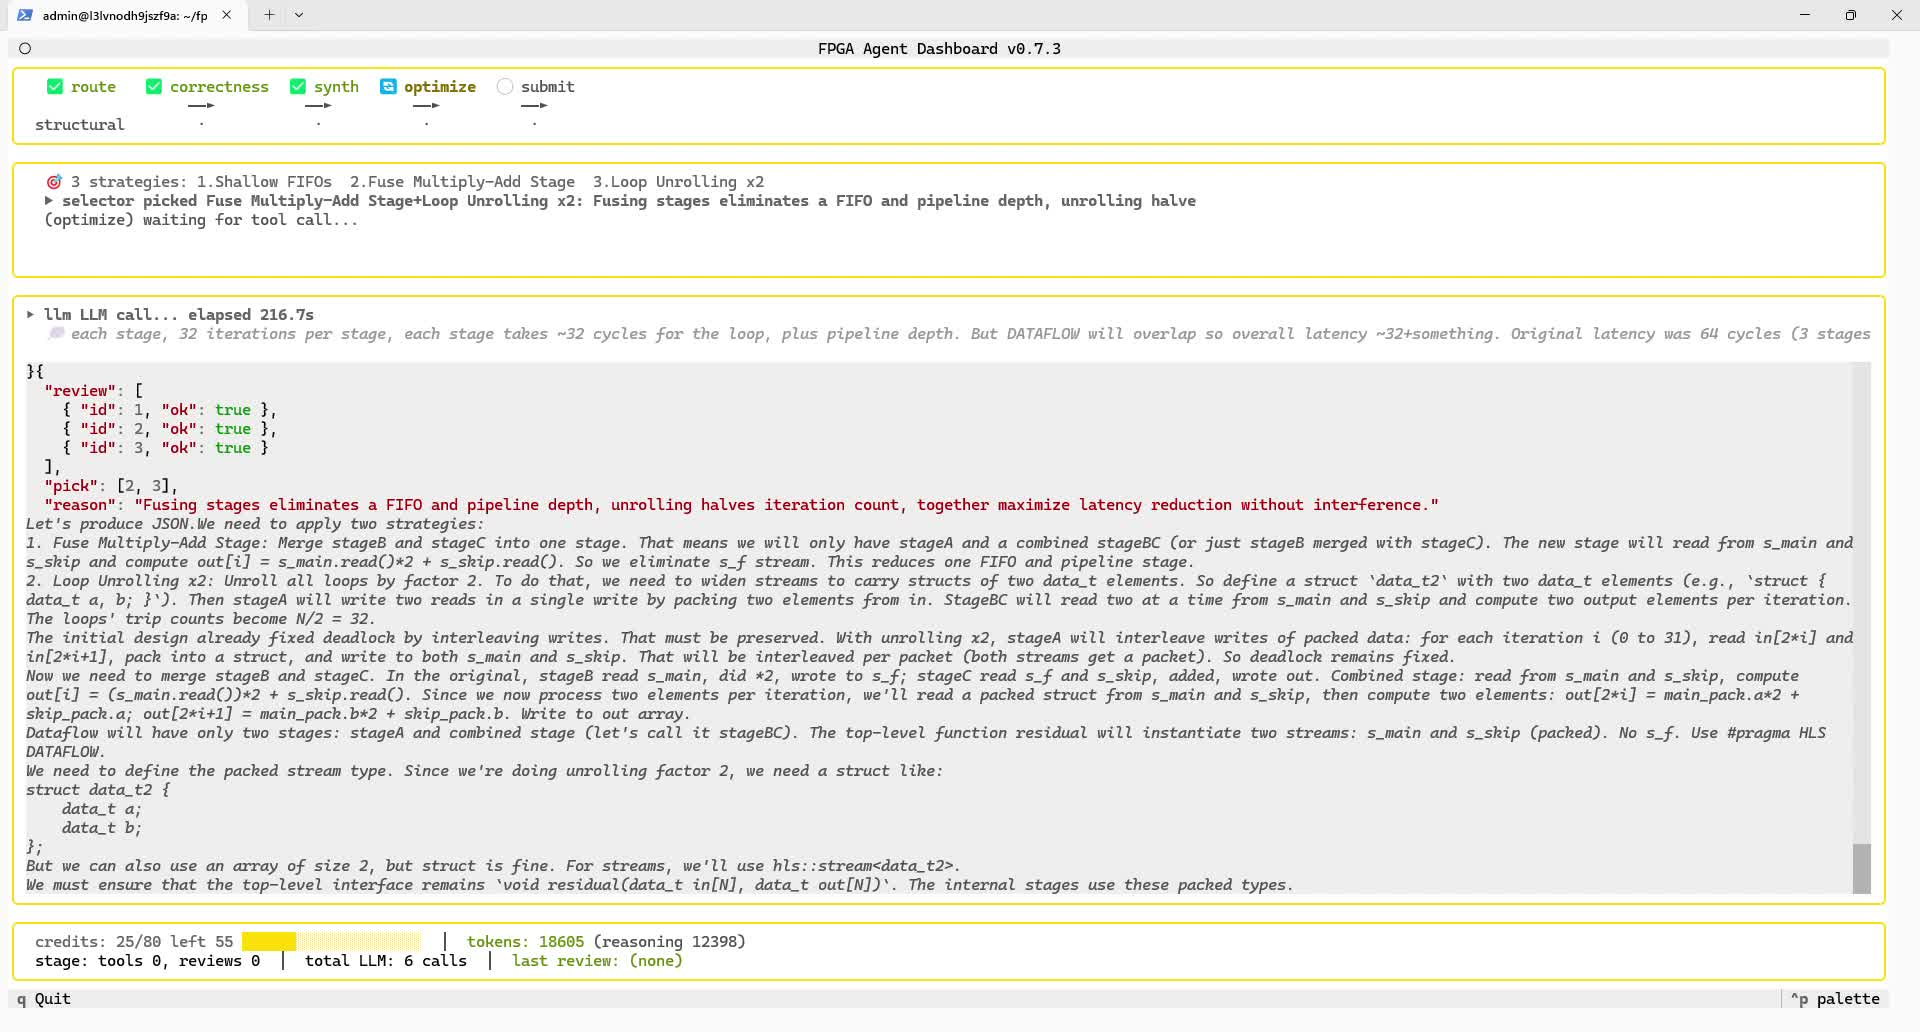
\includegraphics[width=0.95\linewidth]{tui-dashboard.jpg}
\caption{TUI dashboard during a \texttt{dotProduct\_optimize} run.}
\label{fig:tui}
\end{figure}

\end{document}
